\documentclass[10pt]{article}
\usepackage[margin=1in, paperwidth=8.5in, paperheight=11in]{geometry}
\usepackage{ifpdf,amsmath, amssymb, comment, color, graphicx, stmaryrd,setspace,enumitem,tikz, fancyhdr, wrapfig, textcomp, units, mathptmx, pdfpages, cancel, multicol}
\usepackage{hyperref}
\hypersetup{
    colorlinks=true,
    urlcolor=blue,
}

\setlength{\headheight}{14.5pt}
\newcommand{\Q}{\mathbb{Q}}
\newcommand{\R}{\mathbb{R}}
\newcommand{\Z}{\mathbb{Z}}
\newcommand{\vu}{\mathbf{u}}
\newcommand{\vv}{\mathbf{v}}
\newcommand{\vw}{\mathbf{w}}
\newcommand{\vi}{\mathbf{i}}
\newcommand{\vj}{\mathbf{j}}
\newcommand{\vk}{\mathbf{k}}
\newcommand{\vn}{\mathbf{n}}
\newcommand{\vr}{\mathbf{r}}
\newcommand{\va}{\mathbf{a}}
\newcommand{\vF}{\mathbf{F}}
\newcommand{\vL}{\mathbf{L}}
\newcommand{\vT}{\mathbf{T}}
\newcommand{\vN}{\mathbf{N}}
\newcommand{\proj}{\operatorname{proj}}
\newcommand{\orth}{\operatorname{orth}}
\newcommand\del\nabla
\newcommand\dotp[1][.5]{\,\mathbin{\vcenter{\hbox{\scalebox{#1}{$\bullet$}}}}\,}
\newcommand{\slice}{_\text{slice}}

% Solution text is in red. If you want the solutions to show, remove the \iffalse from the definition of the \red command.
%\newcommand{\red}[1]{ %\iffalse
%	\textcolor{red}{#1} }%\fi}

\newenvironment{red}{\color{red}}{\ignorespacesafterend}
\newenvironment{blue}{\color{blue}}{\ignorespacesafterend}
\newcommand{\green}[1]{\textcolor{green}{#1}}
\renewcommand{\section}[1]{\begin{center} \textbf{#1} \\\end{center}}
%
\hyphenpenalty=5000
\setlength{\parindent}{0in}
%\oddsidemargin=-.25in
\allowdisplaybreaks
\pagestyle{fancy}
\renewcommand{\headrulewidth}{0pt}
\lhead{MATH 202}
\rhead{Fall 2022}
%\lfoot{\copyright\ CLEAR Calculus 2010}
\cfoot{}

\begin{document}
%


%\onehalfspacing
\allowdisplaybreaks
%##################################################################
\section{PS\#7: Physics applications; improper integrals - \red{Answer key} }

\everymath{\displaystyle}
\begin{enumerate}[leftmargin=0pt]


\item (\href{https://activecalculus.org/single/sec-6-4-physics.html#wrN}{AC 6.4 Exercise 7}) A cylindrical tank, buried on its side, has radius 3 feet and length 10 feet. It is filled completely with water whose weight density is 62.4 lbs/ft$^3$, and the top of the tank is two feet underground.
\begin{enumerate}
    \item Set up, but do not evaluate, an integral expression that represents the amount of work required to empty the top half of the water in the tank to a truck whose tank lies 4.5 feet above ground.
    
    \begin{red}
    First step: draw a picture and draw a slice. Your picture may of course be a little different -- perhaps in particular you may have chosen to draw a length down from the top of the tank to the slice, rather than the length I've drawn from the center up to the slice. I have both a picture of the overall tank situation and a picture of the end of the tank to help me figure out the relationship between the width of the slice and its height up from the center.
    
    \begin{center}
        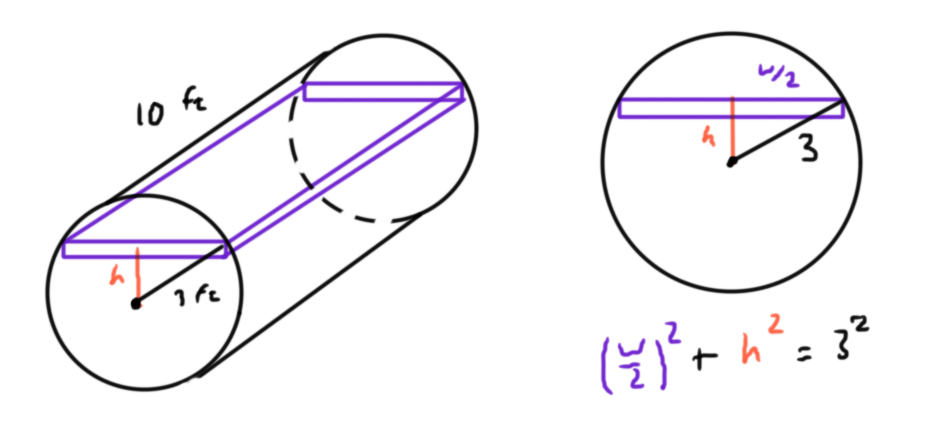
\includegraphics[width=0.7\textwidth]{images/fig-6.4.7.a.png}
    \end{center}
    Now we can figure out the work done to lift a slice. Notice that I'm using capital $W$ for ``work'' and lowercase $w$ for ``width'' -- this is moderately annoying but I believe in you. The work done to lift a slice is the force needed to lift the slice times the distance that slice will be lifted:
    \begin{align*}
        W\slice &= F\slice \cdot d\slice \\
        &= (V\slice\cdot\rho)\cdot d\slice \\ 
        &= (\ell\cdot w\slice \cdot \Delta h\cdot 62.4)\cdot d\slice \\
        \intertext{The width of the slice depends on $h$ in the way illustrated in the diagram. I've solved the equation I wrote for $w$:}
        &= (10\cdot 2\sqrt{9-h^2}\cdot \Delta h \cdot 62.4)\cdot d\slice \\
        \intertext{The slice at height $h$ needs to be lifted by $3-h$ to get to the top of the tank, then by 2 to get to ground level, then by 4.5 to get into the truck.}
        &= (10\cdot 2\sqrt{9-h^2}\cdot \Delta h \cdot 62.4)\cdot (3-h+2+4.5) \\
        &= (10\cdot 2\sqrt{9-h^2}\cdot \Delta h \cdot 62.4)\cdot (9.5-h) \\
        \text{Unit check:\quad \quad} 
        &= (\underbrace{10\cdot}_{\text{ft}}
        \underbrace{2\sqrt{9-h^2}}_{\text{ft}}\cdot 
        \underbrace{\Delta h}_{\text{ft}} \cdot 
        \underbrace{62.4}_{\text{lb / ft}^3})\cdot 
        \underbrace{(9.5-h)}_{\text{ft}} \quad \text{Yay, that's the right units.}
    \end{align*}
    Now we need to integrate from the center of the tank to the top of the tank. That's from $h=0$ to $h=3$. Therefore, the integral computing the amount of work is
    \[W_\text{total} = \int_{h=0}^3 (10\cdot 2\sqrt{9-h^2} \cdot 62.4)\cdot (9.5-h)\ dh.  \]
    \end{red}
    
    \item With the tank now only half-full, set up, but do not evaluate an integral expression that represents the total force due to hydrostatic pressure against one end of the tank.
    
    \begin{red}
    First step: draw a picture and draw a slice. Your picture may of course be a little different -- perhaps in particular you may have chosen to draw a length up from the bottom of the tank to the slice, rather than the length I've drawn from the center down to the slice. 
    
    \begin{center}
        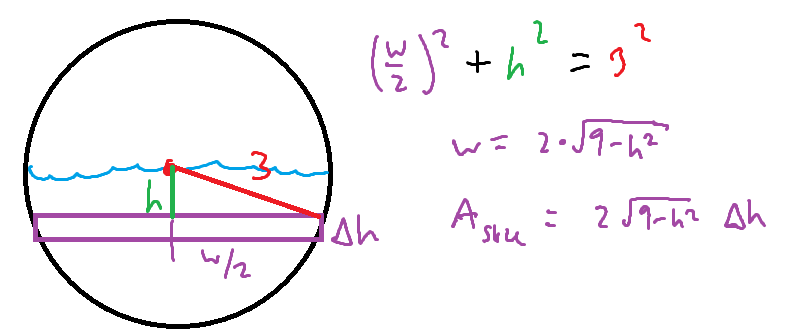
\includegraphics[width=0.7\textwidth]{images/fig-6.4.7.b.png}
    \end{center}
    Now we can figure out the force due to pressure on that slice, which is the area of that slice multiplied by the pressure on that slice. To compute the pressure, we'll multiply the depth of the slice (which is $h$ according to my diagram, since I'm measuring down from the middle) by the weight of water.
    \begin{align*}
        F\slice &= P\slice \cdot A\slice \\
        &= 62.4\cdot h\cdot A\slice \\ 
        &= 62.4\cdot h \cdot (w\slice\cdot\Delta h) \\
        \intertext{The width of the slice depends on $h$ in the way illustrated in the diagram. I've solved the equation I wrote for $w$:}
        &= 62.4\cdot h \cdot \left(2\sqrt{9-h^2}\cdot \Delta h\right)\\
        \text{Unit check:\quad \quad} 
        &= 
        \underbrace{62.4}_{\text{lb / ft}^3}\cdot
        \underbrace{h}_{\text{ft}}\cdot
        \underbrace{2\sqrt{9-h^2}}_{\text{ft}}\cdot
        \underbrace{\Delta h}_{\text{ft}}
         \quad \text{Yay, that's the right units.}
    \end{align*}
    Now we need to integrate from the center of the tank to the bottom of the tank. According to my diagram, that's from $h=0$ to $h=3$. Therefore, the integral computing the amount of work is
    \[F_\text{total} = \int_{h=0}^3 62.4\cdot h \cdot \left(2\sqrt{9-h^2}\right)\ dh.  \]
    \end{red}
\end{enumerate}

\item (\href{https://activecalculus.org/single/sec-6-5-improper.html#IZN}{Activity 6.5.4}) For each of the following definite integrals, decide whether the integral is improper or not. If the integral is proper, evaluate it using the First FTC. If the integral is improper, determine whether or not the integral converges or diverges; if the integral converges, find its exact value.
\begin{enumerate}
    \item $\displaystyle \int_0^1 \frac{1}{x^{1/3}} \, dx$
    
    \begin{red}
    This integral is improper because it is infinitely tall: the integrand has a vertical asymptote at $x=0$, which is included in the bounds of integration. Since this is a $p$-integral with $p < 1$, I know the integral is going to converge. Let's figure out what it converges to:
    %
    \begin{align*}
        \int_0^1 \frac{1}{x^{1/3}} &= 
        \lim_{a\to 0}\int_a^1 \frac1{x^{1/3}}\, dx =
        \lim_{a\to 0}\int_a^1 x^{-1/3}\, dx \\
        &= \lim_{a\to 0} \left[ \frac{x^{2/3}}{2/3} \right|_a^1 
        = \lim_{a\to 0}\left[\frac{1^{2/3}}{2/3} - \frac{a^{2/3}}{2/3}\right] = \frac{3}{2} - 0 = \frac{3}{2}.
    \end{align*}
    \end{red}
    \item $\displaystyle \int_0^2 e^{-x} \, dx$
    
    \begin{red}
    This integral is proper: it is neither infinitely long nor infinitely tall. So finding its value is straightforward:
    \[\int_0^2 e^{-x} \, dx = \left.\vphantom{\int} -e^{-x}\right|_0^2 = -e^{-2} - (-e^{-0}) = -e^{-2}+1.\]
    \end{red}
    \item $\displaystyle \int_1^4 \frac{1}{\sqrt{4-x}} \, dx$
    
    \begin{red}
    This integral is improper because it is infinitely tall: the integrand has a vertical asymptote at $x=4$, which is included in the bounds of integration. I'm pretty sure this is going to converge because the power is $1/2 < 1$, but in order to figure out what it converges to, we'll need to do a substitution $u = 4-x$, $du = -dx$:
    \begin{align*}
        \int_1^4 \frac{1}{\sqrt{4-x}} \, dx &= \lim_{b\to 4}\int_1^b \frac{1}{\sqrt{4-x}}\, dx \\
        &= \lim_{b\to 4}\int_{x=1}^{x=b} \frac{1}{\sqrt{u}}\, (-du) 
        = -\lim_{b\to 4}\int_{x=1}^{x=b} u^{-1/2}\, du \\
        &= -\lim_{b\to 4}\left[ \frac{u^{1/2}}{1/2} \right|_{x=1}^{x=b}
        \intertext{Now we back-substitute before plugging in the bounds of integration so that we do not make a puppy cry:}
        &= -\lim_{b\to 4}\left[ \frac{(4-x)^{1/2}}{1/2} \right|_1^b 
        = -\lim_{b\to 4}\left[ \frac{(4-b)^{1/2}}{1/2} - \frac{3^{1/2}}{1/2} \right]
        = -(0 - 2\sqrt{3}) = 2\sqrt{3}.
    \end{align*}
    \end{red}
    
    \item $\displaystyle \int_{-2}^2 \frac{1}{x^2} \, dx$
    
    \begin{red}
    This integral is sneakily improper because the integrand has a vertical asymptote at 0, which is included in the bounds of integration, so the region is infinitely tall. Since this is a $p$-integral with $p > 2$, the integral will diverge. Let's see why:
    \[\int_{-2}^2 \frac{1}{x^2}\, dx = \int_{-2}^0 \frac{1}{x^2}\, dx + \int_0^2 \frac{1}{x^2}\, dx\]
    Here I'm going to play a trick: Look at a graph of $\frac{1}{x^2}$ and notice that it is symmetric across the $y$-axis. Therefore, these two integrals I've set up will have the same value, so I'm just going to calculate one of them and double it.
    \[ = 2\int_0^2 \frac{1}{x^2}\, dx = 2\lim_{a\to 0} \int_a^2 x^{-2}\, dx = 2\lim_{a\to 0} \left.\frac{x^{-1}}{-1} \right|_a^2 = 2\lim_{a \to 0}\left(\frac{-1}{2} - \frac{-1}{a}\right) \]
    In the limit as $a$ approaches 0, $\frac{1}{a}$ will increase without bound. Therefore, this integral diverges. 
    \end{red}
    \item $\displaystyle \int_0^{\pi/2} \tan(x) \, dx$
    
    \begin{red}
    This integral is sneakily improper because the integrand has a vertical asymptote at $\pi/2$, which is included in the bounds of integration, so the region is infinitely tall. If you happen to remember that $\int\tan(x)\, dx = \ln|\cos(x)| +C$, you could use that fact, but let's do it by substitution because that's more fun:
    %
    \begin{align*}
        \int_0^{\pi/2} \tan(x)\ dx 
        &= \int_0^{\pi/2} \frac{\sin(x)}{\cos(x)}\ dx 
        = \lim_{b\to \pi/2}\int_0^b\frac{\sin(x)}{\cos(x)}\ dx
        \intertext{So let's substitute $u = \cos(x)$, $du = \sin(x)\ dx$:}
        &= \lim_{b\to \pi/2}\int_{x=0}^{x=b} \frac{1}{u}\ du 
        = \left.\lim_{b\to \pi/2} \ln|u| \right|_{x=0}^{x=b}
        = \left.\lim_{b\to \pi/2} \ln|\cos(x)| \right|_0^b \\
        &= \lim_{b\to \pi/2} \left(\vphantom\int \ln|\cos(b)| - \ln|\cos(0)|\right)
        = \lim_{b\to \pi/2} \left(\vphantom\int\ln|\cos(b)| - \ln(1)\right) \\
        &= \lim_{b\to \pi/2} \left(\vphantom\int \ln|\cos(b)| - 0\right)
    \end{align*}
    And now we see a problem: as $b\to \pi/2$, $\cos(b) \to 0$, and so $\ln|\cos(b)| \to -\infty$. Therefore this integral diverges.
    \end{red}
    \item $\displaystyle \int_0^1 \frac{1}{\sqrt{1-x^2}} \, dx$
    
    \begin{red}
    This integral is infinitely tall because the integrand has a vertical asymptote at $x=1$, which is included in the bounds of integration. 
    %
    \begin{align*}
        \int_0^1\frac{1}{\sqrt{1-x^2}}\ dx 
        &= \lim_{b\to 1} \int_0^b \frac{1}{\sqrt{1-x^2}}\ dx = \lim_{b\to 1}\left[\vphantom\int \arcsin(x)\right|_0^b \\
        &= \lim_{b\to 1} \left[\vphantom\int \arcsin(b) - \arcsin(0) \right] 
        = \arcsin(1) - \arcsin(0) = \frac{\pi}{2} - 0 = \frac{\pi}{2}.
    \end{align*}
    \end{red}
\end{enumerate}

\end{enumerate}
\end{document}